\documentclass[professionalfonts, xcolor={usenames,svgnames,x11names,table}]{beamer}

\usetheme{SBUclass}
\usepackage{mypackages}
\usepackage{mycommands}


\title{\texorpdfstring{Language \& Technology}{Language and Technology}}
\subtitle{Lecture 7: From Unigrams to n-Grams}
\author{Al{\"e}na Aks{\"e}nova \& Aniello De Santo}
\institute{Stony Brook University\\\texttt{alena.aksenova@stonybrook.edu}\\\texttt{aniello.desanto@stonybrook.edu}}
\date{}


\unnumbered{
\begin{document}
\begin{frame}{Plan for Remaining 5 Weeks}
    \centering
    \begin{tabular}{rll}
        \toprule
        \textbf{Date} & \textbf{Topic} & \textbf{Hw?}\\
        \midrule
       April  8  & n-gram models & yes\\
       April  10  & Python (functions) \\
        \midrule
        April  15 &  n-gram models (cont.) & yes\\
       April  17 & Python (tokens) \\
        \midrule
       April 22 & Machine learning &yes \\
        April  24 & Python (ngrams)\\
        \midrule
       April  29 &  Human-like models  & practice /Final project  \\
       May 01 & Python (frequencies)\\
        \midrule
        May 06 & Summary & Final project  \\
        May 08 & Python Q\&A session\\
            \midrule
        May 14 & & Final Project due (at midnight)\\
        
        \bottomrule
    \end{tabular}
\end{frame}

%\begin{frame}{Learning More}
%    Related courses in the spring:
%
%    \begin{itemize}
%        \item \textbf{Syntax (LIN 311)}\\
%            Prerequisite: Lin 101
%        \item \textbf{Parsing and Processing (Lin 630)}\\
%            Graduate level!\\
%            Prerequisite: Lin 311, having done well in this course
%        \item \textbf{Revising my MathMethods Lecture Notes}\\
%            Prerequisite: reliability and independence\\
%            SBC: EXP+
%    \end{itemize}
%\end{frame}
}

\unnumbered{
\begin{frame}
	\titlepage
\end{frame}
}



\begin{frame}{Generalizing Unigrams}
    \begin{itemize}
        \item Unigram models perform reasonably well:
            \begin{itemize}
                \item cultuormics
                \item stylistic analysis
                \item authorship attribution
                \item word semantics
                \item ad placement
                \item web search
            \end{itemize}
        \item But they only consider words in isolation.
        \item An n-gram model looks at \highlight{sequences of words}.
    \end{itemize}
\end{frame}

\begin{frame}{Example: Word Prediction}
    Your phone can make suggestions for the most likely next word(s).

    \begin{block}{A (Bad) Solution with Unigrams}
       \begin{enumerate}
            \item Build corpus.
            \item For each word type, calculate number of tokens.
            \item Calculate the \highlight{frequency} of the word in the sample:
                \[
                    \text{freq}(
                        \text{\colored{blue!75}{\emph{word}}},
                        \text{\colored{orange}{\emph{sample}}}
                        )
                    =
                    \frac{%
                        \text{number of tokens of \colored{blue!75}{\emph{word}}}}
                        {\text{word length of whole \colored{orange}{\emph{sample}}}}
                \]
            \item Suggest words with highest frequency.
       \end{enumerate} 
    \end{block}
\end{frame}

\begin{frame}{Example Calculation}
    \textbf{Sample:} \colored{SteelBlue4}{1000} words long
    \hfill
    \textbf{Words:} be, bed, bee, bell
    %
    \begin{center}
        \begin{tabular}{rcccc}
            \textbf{Type} & be & bed & bee & bell\\
            \textbf{Tokens} & \color{orange}\bfseries 13 & \color{purple}\bfseries 2 & \color{SeaGreen4}\bfseries 0 & \color{brown}\bfseries 3 
        \end{tabular}
    \end{center}
    %
    \[
        \begin{array}{c@{\hspace{2em}}c}
            \text{freq}(\text{be}) = \frac{\color{orange}\mathbf{13}}{\color{SteelBlue4} 1000} = 1.3\%
            &
            \text{freq}(\text{bee}) = \frac{\color{SeaGreen4}\mathbf{0}}{\color{SteelBlue4} 1000} = 0.0\%
            \\[6pt]
            \text{freq}(\text{bed}) = \frac{\color{purple}\mathbf{2}}{\color{SteelBlue4} 1000} = 0.2\%
            &
            \text{freq}(\text{bell}) = \frac{\color{brown}\mathbf{3}}{\color{SteelBlue4} 1000} = 0.3\%\\
        \end{array}
    \]
\end{frame}

\begin{frame}{This is a Workable Solution for Word Completion}
    \begin{description}
        \item[word completion] completing a partially typed word
    \end{description}

    A frequency-based unigram model can work reasonably well\\
    for word completion.

    \begin{example}
    \[
        \begin{array}{c@{\hspace{2em}}c}
            \text{freq}(\text{be}) = \frac{\color{orange}\mathbf{13}}{\color{SteelBlue4} 1000} = 1.3\%
            &
            \text{freq}(\text{bee}) = \frac{\color{SeaGreen4}\mathbf{0}}{\color{SteelBlue4} 1000} = 0.0\%
            \\[6pt]
            \text{freq}(\text{bed}) = \frac{\color{purple}\mathbf{2}}{\color{SteelBlue4} 1000} = 0.2\%
            &
            \text{freq}(\text{bell}) = \frac{\color{brown}\mathbf{3}}{\color{SteelBlue4} 1000} = 0.3\%\\
        \end{array}
    \]

    \medskip
    \textbf{Partial input:} be\\
    \textbf{Ranked completions:} be, bell, bed, bee
    \end{example}
\end{frame}

\begin{frame}{Why This is a Horrible Solution for Word Prediction}
    \begin{description}
        \item[word prediction] suggesting next word before it is typed
    \end{description}

    Unigram models are horrible for word prediction:
    \begin{itemize}
        \item always suggest  the same words
        \item only suggest stop words (because they're most frequent)
        \item do not take context into account
    \end{itemize}

    \begin{block}{The n-Gram Hypothesis}
        One can reliably predict the next word based on\\
        the \highlight{preceding $n-1$ words}.
    \end{block}
\end{frame}

\begin{frame}{Defining n-grams}
    \begin{description}
        \item[n-gram] a contiguous sequence of $n$ words
    \end{description}

    \begin{center}
        \begin{tabular}{rll}
            \toprule
            \textbf{n} & \textbf{Name} & \textbf{Example}\\
            \midrule
            1 & unigram & John\\
            2 & bigram  & John to\\
            3 & trigram & John to be\\
            4 & 4-gram & John to be in\\
            5 & 5-gram & John to be in the car\\
            \bottomrule
        \end{tabular}
    \end{center}

    \begin{example}
        \textbf{String}\\
        \begin{tikzpicture}
            \matrix (m) at (0,0) [matrix of nodes, ampersand replacement=\&] {%
                John \& and \& Marie \& are \& not \& Bill \& and \& Sue\\
            };
            \begin{pgfonlayer}{background}
                % bigrams
                \foreach \Right [remember=\Right as \previous (initially 1)] in {2,3,4,5,6,7,8}
                    \draw[draw=purple,fill=purple!25,thick,
                          visible on=<\Right>]
                        (m-1-\previous.south west) rectangle (m-1-\Right.north east);

                % trigrams
                \foreach \Left/\Right/\Timer in {%
                    1/3/9,
                    2/4/10,
                    3/5/11,
                    4/6/12,
                    5/7/13,
                    6/8/14%
                    }
                    \draw[draw=blue,fill=blue!25,thick,
                          visible on=<\Timer>]
                        (m-1-\Left.south west) rectangle (m-1-\Right.north east);

                % 4-grams
                \foreach \Left/\Right/\Timer in {%
                    1/4/15,
                    2/5/16,
                    3/6/17,
                    4/7/18,
                    5/8/19%
                    }
                    \draw[draw=brown,fill=brown!25,thick,
                          visible on=<\Timer>]
                        (m-1-\Left.south west) rectangle (m-1-\Right.north east);

                % 5-grams
                \foreach \Left/\Right/\Timer in {%
                    1/5/20,
                    2/6/21,
                    3/7/22,
                    4/8/23%
                    }
                    \draw[draw=teal,fill=teal!25,thick,
                          visible on=<\Timer>]
                        (m-1-\Left.south west) rectangle (m-1-\Right.north east);
            \end{pgfonlayer}
        \end{tikzpicture}
    \end{example}
\end{frame}

\begin{frame}{Frequencies for n-grams}
    Frequencies can be computed for n-grams, too.

    \begin{exampleblock}{Example: Calculating Bigram Frequencies}
        \begin{itemize}
            \item \textbf{String}\\
                \begin{tikzpicture}
                    \matrix (m) at (0,0) [matrix of nodes, ampersand replacement=\&] {%
                        when \& buffalo \& buffalo \& buffalo \& buffalo \& buffalo \& buffalo\\
                    };
                    \begin{pgfonlayer}{background}
                        \foreach \Right [remember=\Right as \previous (initially 1)] in {2,3,4,5,6,7}
                            \draw[draw=purple,fill=purple!25,thick,
                                  visible on=<\Right>]
                                (m-1-\previous.south west) rectangle (m-1-\Right.north east);
                    \end{pgfonlayer}
                \end{tikzpicture}
            %
            \item \textbf{Bigram token list}\\
                \visible<2->{when buffallo,}
                \visible<3->{buffalo buffalo,}
                \visible<4->{buffalo buffalo,}
                \visible<5->{buffalo buffalo,}
                \visible<6->{buffalo buffalo,}
                \visible<7->{buffalo buffalo}
            %
            \item \textbf{Bigram counts and frequencies}\\
                \visible<8>{
                \begin{enumerate}
                    \item when buffalo: 1 $\Rightarrow \frac{1}{6} = 16.7\%$
                    \item buffalo buffalo: 5 $\Rightarrow \frac{5}{6} = 83.3\%$
                \end{enumerate}
                }
        \end{itemize}
    \end{exampleblock}
\end{frame}

\begin{frame}{How Your Phone Does it}
    \begin{itemize}
        \item Frequency database for n-grams ($2 \leq n \leq 5$)
        \item Look at previous $n-1$ words.
        \item Pick \highlight{fitting $n$-gram with highest frequency}.
    \end{itemize}

    \begin{example}
        \begin{itemize}
            \item \textbf{Trigram frequencies}\\
                \begin{tabular}{lr@{\hspace{2em}}lr}
                    bus is late  & 30\% & train is late  & 15\%\\
                    bus is cheap & 25\% & train is cheap & 8\%\\
                    bus is early & 20\% & train is early & 2\%\\
                \end{tabular}
            \item \textbf{Input}\\
                I will text you if the train is
            \item \textbf{Word suggestion}\\
                \visible<2>{late}
        \end{itemize}
    \end{example}
\end{frame}

\begin{frame}{Choosing the right $n$ is Important}

An example from Grammarly ... 
\begin{center}
  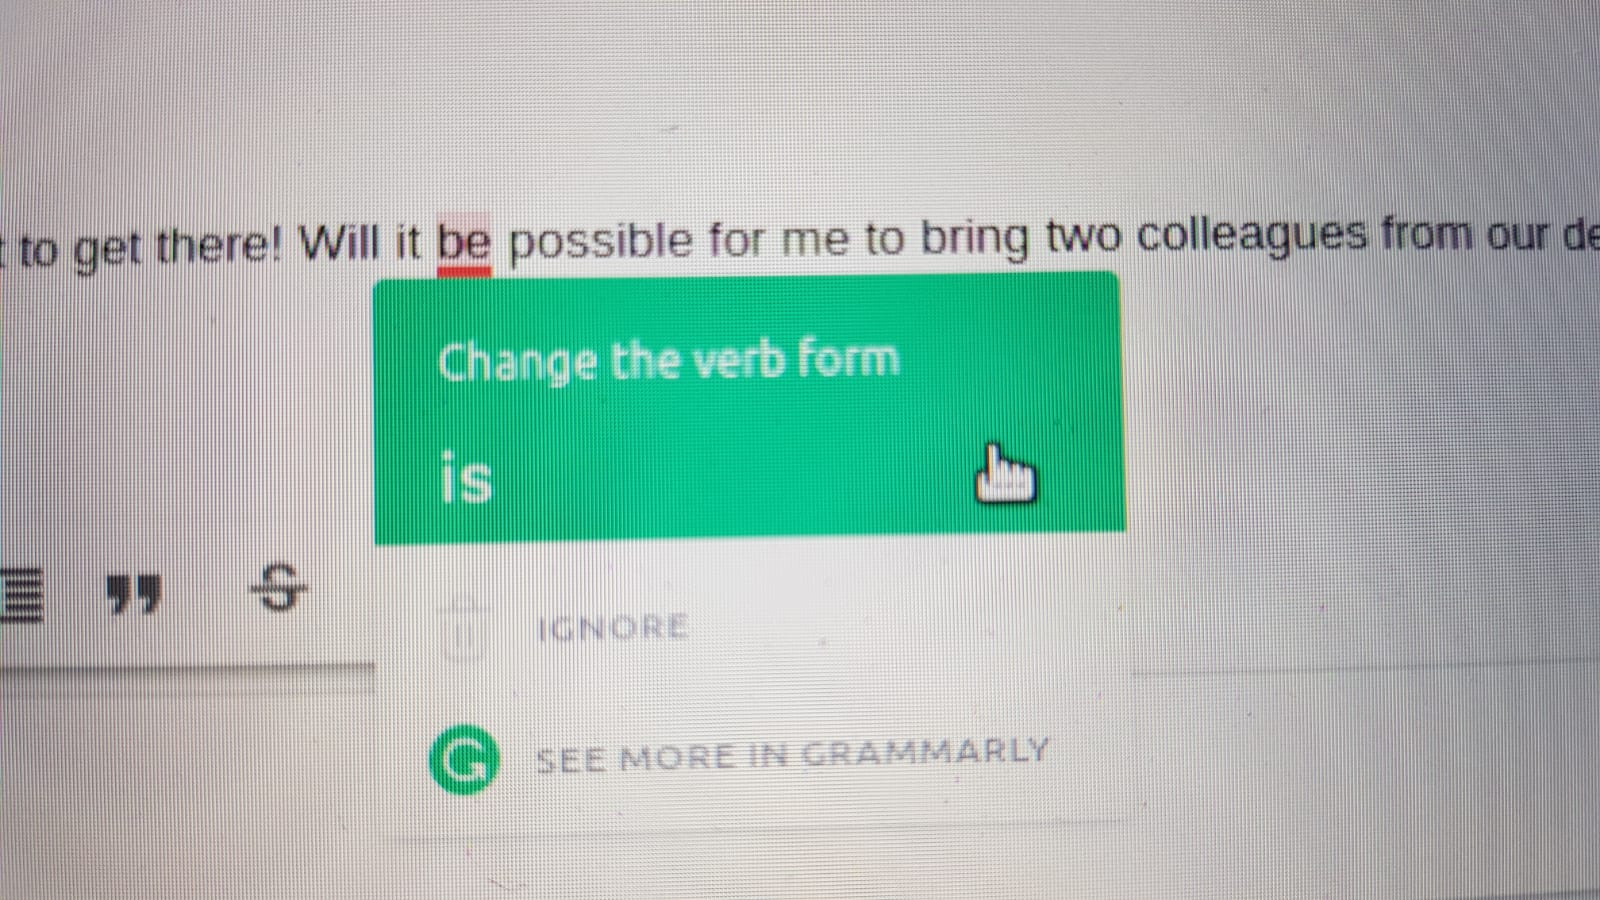
\includegraphics[width=.9\linewidth]{./img/grammarly}
  \end{center}
\end{frame}


\begin{frame}{Zipf's Law Strikes Again}
    \begin{itemize}
        \item As with words, n-grams have a Zipfian distribution.
        \item This creates a major problem: \highlight{sparse data}
    \end{itemize}

    \begin{block}{The Overwhelming Number of $n$-Grams}
        \begin{itemize}
            \item Suppose English has 5,000 words (it actually has way more)
            \item Suppose each word has two inflected forms\\
                \subpoint{\textbf{see the picture} and \textbf{see the pictures} are distinct trigrams!}
            \item Then there are $10,000^n = 10^{4n}$ distinct $n$-grams.
                \begin{center}
                    \begin{tabular}{rl}
                        \toprule
                        \textbf{n} & \textbf{number of possible n-grams}\\
                        \midrule
                        2 & 100 million\\
                        3 & 1 trillion\\
                        4 & 10 quadrillion\\
                        5 & 100 quintillion\\
                        \bottomrule
                    \end{tabular}
                \end{center}
        \end{itemize}
    \end{block}
\end{frame}

\begin{frame}{Is That a Lot?}
    \begin{itemize}
        \item Assuming $10,000$ English word forms, the number of $5$-grams rivals the \highlight{number of seconds since the Big Bang}!
    \end{itemize}

    \begin{block}{The Sparse Data Problem}
        \begin{enumerate}
            \item We want a large $n$ for better accuracy.
            \item But the larger the $n$, the more data we need.
            \item Because of Zipf's law, the majority of the data\\
                    consists of the same $n$-grams. 
            \item Hence most grammatical $n$-grams have a frequency of $0$. 
            \item This means they will never be suggested,\\
                even if there is no grammatical alternative.
        \end{enumerate}
    \end{block}
\end{frame}

\begin{frame}{Things Get Worse: A More Realistic Estimate}
    \begin{itemize}
        \item The Unix dictionary american-english-insane has\\
            650,000 entries.
        \item This makes the numbers much worse.\\
            Can you guess how many 5-grams there are then?
    \end{itemize}

    \begin{center}
        \visible<2->{116 octillion $\mathbf{\approx 10^{29}}$}

        \visible<3->{
            \medskip
            \begin{tabular}{rl}
                \textbf{Number} & \textbf{Real-world counterpart}\\
                $10^{14}$ & distance in millimeters from Earth to Sun\\
                $10^{18}$ & seconds since Big Bang\\
                $10^{24}$ & milliliters of water in the oceans\\
            \end{tabular}
        }
    \end{center}
        
    \medskip
    \visible<4>{
            $10^{29}$ is larger than the number of shotglasses it takes to\\
            drain Earth's oceans over 2000 times.
        }
\end{frame}

\begin{frame}{Trick 1: Stemming and Lemmatization}
    \begin{itemize}
        \item Removing inflectional markers reduces number of words
        \item Two solutions:
            \begin{itemize}
                \item stemming is quick and dirty
                \item lemmatization is accurate but complex
            \end{itemize}
    \end{itemize}

    \begin{description}
        \item[stemming] cut off word ends that look like inflection
    \end{description}

    \begin{example}
        \begin{itemize}
            \item cats $\Rightarrow$ cat
            \item tasks $\Rightarrow$ task (noun and verb)
            \item asking $\Rightarrow$ ask
            \item meeting $\Rightarrow$ meet (\textbf{noun and verb})
        \end{itemize}
    \end{example}
\end{frame}

\begin{frame}{Trick 1: Stemming and Lemmatization [cont.]}
    \begin{description}
        \item[lemmatization] stemming with context information
    \end{description}

    \begin{example}
        \begin{itemize}
            \item cats $\Rightarrow$ cat
            \item tasks $\Rightarrow$ task (noun and verb)
            \item asking $\Rightarrow$ ask
            \item meeting $\Rightarrow$ meet (\textbf{only verb})
        \end{itemize}
    \end{example}

    \begin{block}{Evaluation}
        \begin{itemize}
            \item Stemming\slash lemmatization reduces the number of words.
            \item But we still have at least 10,000 words and thus $10^{20}$ 5-grams.
        \end{itemize}
    \end{block}
\end{frame}

\begin{frame}{Trick 2: Statistics}
    \begin{itemize}
        \item \textbf{Backoff Method}\\
            If an $n$-gram has frequency $0$, use the frequency of the corresponding $(n-1)$-gram.
        \item \textbf{Good-Turing Smoothing}\\
            Change frequency from $0$ to a very low value while lowering high frequency values.
    \end{itemize}

    \begin{block}{Evaluation}
        \begin{itemize}
            \item These tricks solve the issue of n-grams with 0\% frequency.
            \item But they do not solve the basic problem that n-gram models are incredibly data hungry.
        \end{itemize}
    \end{block}
\end{frame}

\begin{frame}{Future of n-Gram Models}
    \begin{itemize}
        \item Moving from unigrams to n-gram models increases performance in many applications we discussed.
            \begin{itemize}
                \item culturomics
                \item stylistic analysis
                \item web search
                \item ad placement
            \end{itemize}
        \item But we quickly hit diminishing returns.
        \item Even 5-gram models are \highlight{no match for humans}, and it's unlikely we'll be able to move on to 6-grams any time soon.
    \end{itemize}
\end{frame}

\begin{frame}{New Areas of Application}
    \begin{itemize}
        \item N-gram models are nearly maxed out in current applications.
        \item But this still leaves areas where they haven't been used at all.
        \item Let's briefly look at one example: OCR.
    \end{itemize}
\end{frame}

\begin{frame}{Optical Character Recognition}
    \begin{description}
        \item[OCR] the process of
            \begin{enumerate}
                \item scanning in images of text and
                \item converting it into digital text.
            \end{enumerate}
            ``making computers read''
    \end{description}

    \begin{itemize}
        \item In a purely digital world, OCR would be superfluous.
        \item But there's still many analog texts that need to be digitized.\\
            \subpoint{old books, paper forms, signed contracts, \ldots}
        \item A special (and much harder) case of OCR is\\
            handwriting recognition.\\
    \end{itemize}
\end{frame}

\begin{frame}{The Quality of Current OCR Software}
    \begin{itemize}
        \item OCR sounds trivial; even a 4-year old can recognize letters
        \item So \highlight{why are my ebooks full of mistakes?}
    \end{itemize}
    %
    \begin{columns}
        \column{.65\linewidth} 
        \begin{exampleblock}{Examples from \emph{Diaspora} (1997)}
            \begin{itemize}
                \item That was-n't entirely true;
                \item 1 want sharp borders, right now.
                \item The carpets seem to he vulnerable.
                \item If they can shorten wormholes, the$\backslash$, might visit us.
                \item He fell silent, abruptly realizing "it'll she t, as feeling: electing not to wake up again [\ldots]
                \item Seaweed every twenty -seven -seven I DIASPORA 231 light years.
            \end{itemize}
        \end{exampleblock}

        \column{.35\linewidth} 
        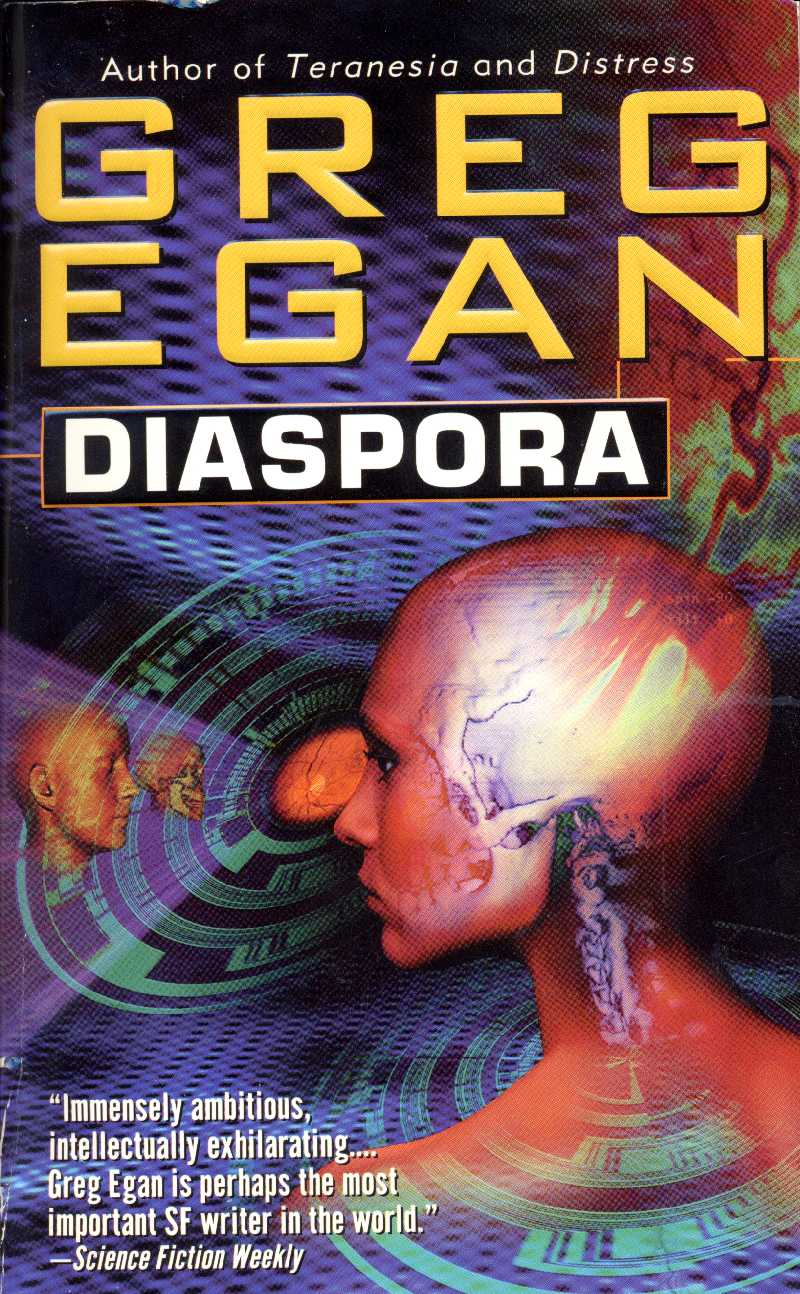
\includegraphics[width=.9\linewidth]{./img/diaspora}
    \end{columns}
\end{frame}

\begin{frame}{The Prototype Problem}
    \begin{itemize}
        \item Characters have \highlight{prototypical shapes}.
        \item But numerous deviations are possible, with fuzzy borders.
    \end{itemize}
    %
    \begin{exampleblock}{Non-Mandatory Properties of the Letter A}
        \begin{columns}
            \column{.6\linewidth}
            \begin{itemize}
                \item two angular strokes, meeting at top
                \item cross bar
                \item no horizontal top stroke
                \item no horizontal bottom stroke
                \item no curves or arcs
                \item no disconnected parts
            \end{itemize}
            
            \column{.4\linewidth}
            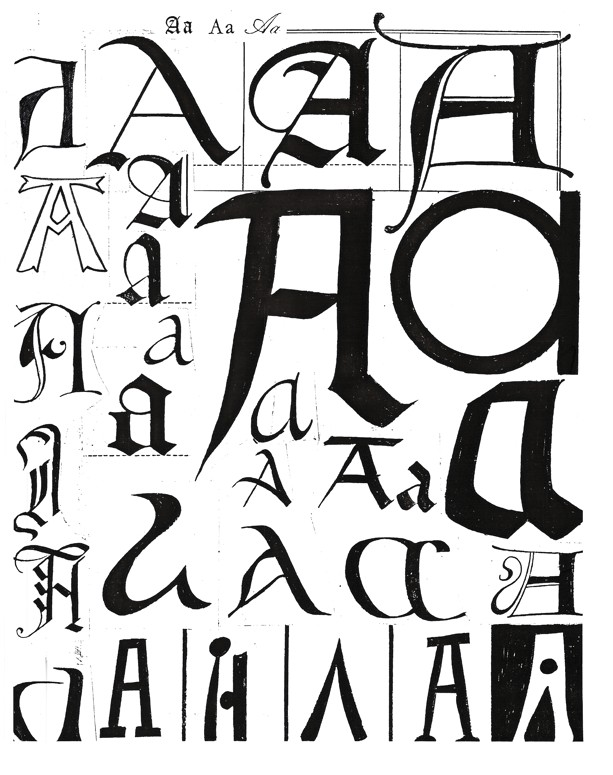
\includegraphics[width=.9\linewidth]{./img/lettera}
        \end{columns}
    \end{exampleblock}
\end{frame}

\begin{frame}{Recognizing Characters is Not Enough}
    \begin{itemize}
        \item Mapping pixels in an image to characters is a probabilistic process that is affected by many parameters
            %
            \begin{itemize}
                \item font
                \item low-quality printing process
                \item stains on page
                \item[$\vdots$]
            \end{itemize}
            %
        \item Some misidentifications are unavoidable.
        \item Why don't humans run into the same problems?\\
            Because \highlight{humans do not read character by character}.
    \end{itemize}
\end{frame}

\begin{frame}{Basic Properties of Human Reading}
    \begin{itemize}
        \item \textbf{Saccades}\\
            reading proceeds not character by character,\\
            eyes move in \highlight{saccades}:
            \begin{enumerate}
                \item focus on several words at once and identify words,
                \item once done, move eyes to next cluster of words to the right,
                \item focus, absorb, then move again, and so on.
            \end{enumerate}
            %
        \item \textbf{Word Identification}\\
            pattern-match whole words rather than character sequences\\
            $\Rightarrow$ order of character usually of little relevance
            %
            \begin{center}
                \colored{teal}{I cnduo't bvleiee taht I culod aulaclty uesdtannrd\\ waht I was rdnaieg.}
            \end{center}
            %
        \item \textbf{Predictive}\\
            speakers use information about sentence to predict next word\\
            $\Rightarrow$ unexpected words read more slowly
    \end{itemize}
\end{frame}

\begin{frame}{Taking a Hint: Adding Unigrams to OCR}
    \textbf{Proposal:} OCR-ed sequence of characters must be\\
    a word in our dictionary

    \begin{exampleblock}{Examples from \emph{Diaspora} (1997)}
        \begin{itemize}
            \item \Strikeout{1}{2-}{That was-n't entirely true;}
            \item 1 want sharp borders, right now.
            \item The carpets seem to he vulnerable.
            \item \Strikeout{-2}{3-}{If they can shorten wormholes, the$\backslash$, might visit us.}
            \item \Strikeout{-3}{4-}{He fell silent, abruptly realizing "it'll she t, as feeling: electing not to wake up again [\ldots]}
            \item Seaweed every twenty seven seven I DIASPORA 231 light years.
        \end{itemize}
    \end{exampleblock}
\end{frame}

\begin{frame}{Taking a Hint: Adding Bigrams to OCR}
    \textbf{Proposal:} only pick words that yield licit bigram
    
    \begin{exampleblock}{Examples from \emph{Diaspora} (1997)}
        \begin{itemize}
            \item \Strikeout{0}{1-}{That was-n't entirely true;}
            \item \Strikeout{1}{2-}{1 want sharp borders, right now.}
            \item \Strikeout{-2}{3-}{The carpets seem to he vulnerable.}
            \item \Strikeout{0}{1-}{If they can shorten wormholes, the$\backslash$, might visit us.}
            \item \Strikeout{0}{1-}{He fell silent, abruptly realizing "it'll she t, as feeling: electing not to wake up again [\ldots]}
            \item \Strikeout{-3}{4}{Seaweed every twenty seven seven I DIASPORA 231 light years.}
        \end{itemize}
    \end{exampleblock}
\end{frame}

\begin{frame}{Problems of the Approach}
    Why don't OCR models use $n$-grams?\\
    They \highlight{create new problems}.

    \begin{columns}
        \column{.7\linewidth}

        \begin{itemize}
            \item Lexical creativity\\
                \subpoint{Neal Stephensons's \emph{Anathem}: speely captor, jeejah, fraa, suur, cartabla, orth, saunt, suvin}
            \item Grammatical creativity\\
                \subpoint{\emph{Diaspora:} gender-neutral pronoun ve\slash vis\slash ver} 
            \item (Deliberately) Archaic language\\
                \subpoint{Tolkien's \emph{LotR}: anon, askance, ere, furlong, lissom, recreant, thraldom}
            \item Multiple languages\\
                \subpoint{German and French in \emph{The Magic Mountain}}
            \item Typos
        \end{itemize}

        \column{.3\linewidth}
        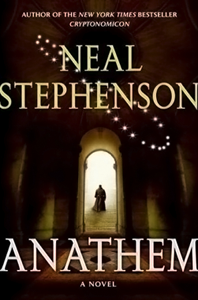
\includegraphics[width=.9\linewidth]{./img/anathem}
    \end{columns}
\end{frame}

\begin{frame}{Summary: OCR Needs Fixing}
    \begin{itemize}
        \item Current OCR models operate purely character-by-character.
        \item They do not produce stellar results.\\
              \subpoint{even 99\% accuracy means at least one mistake every other page}
        \item Humans are much more competent and use linguistic insights.
        \item Adding $n$-grams is a first step in the same direction.
    \end{itemize}
\end{frame}

\end{document}
